\usetikzlibrary{positioning}
\usetikzlibrary{shapes,arrows}
\tikzstyle{block} = [draw, fill=blue!20, rectangle, 
    minimum height=3em, minimum width=2em]
\tikzstyle{sum} = [draw, fill=blue!20, circle, node distance=1cm]
\tikzstyle{input} = [coordinate]
\tikzstyle{output} = [coordinate]   
\tikzstyle{pinstyle} = [pin edge={to-,thin,black}]

\tikzstyle{blockbig} = [draw, fill=white, rectangle, 
    minimum height=6em, minimum width=3em]
\tikzset{
block/.style = {draw, fill=white, rectangle, minimum height=3em, minimum width=3em},
tmp/.style  = {coordinate}, 
sum/.style= {draw, fill=white, circle, node distance=1cm},
input/.style = {coordinate},
output/.style= {coordinate},
pinstyle/.style = {pin edge={to-,thin,black}}
}



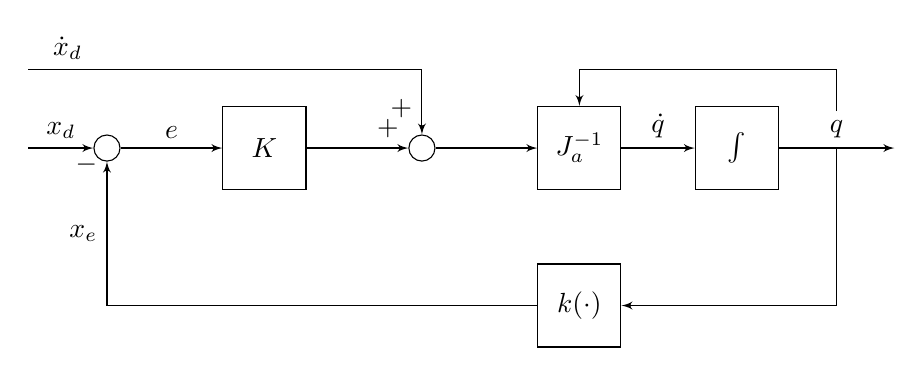
\begin{tikzpicture}[auto, node distance=2cm,>=latex']
    % We start by placing the blocks
    \node  [input, name=input2] {};
    \node at (0,-1) [input, name=input] {};
    \node [sum, right of=input] (sum) {};
    \node [block, right of=sum] (K) {${K}$};
    \node [sum, right of=K, node distance=2cm] (sum2) {};
    \node [tmp, above of =sum2, node distance=1cm] (tmp1){};
    \node [block, right of=sum2] (JA) {${J}_a^{-1}$};
    \node [block, below of=JA] (k) {${k}(\cdot)$};
    \node [block, right of=JA] (Integral) {$\int$};
    \node [tmp, above of=JA, node distance=1cm] (tmp2){};
    \node [output, right of=Integral] (output) {};

    % Once the nodes are placed, connecting them is easy. 
    \draw [draw,->] (input) -- node {${x}_d$} (sum);
    %\draw [draw,->] (input2) -- node {$u$} (sum2);
    \draw [draw,->] (input2) -- node [pos=0.1] {${\dot{x}}_d$} (tmp1)-| node [pos=0.8,anchor=left,left] {$+$} (sum2);
    \draw [->] (sum) -- node {${e}$} (K);
    \draw [->] (K) -- node {}  node[pos=0.8] {$+$} (sum2);
    \draw [->] (sum2) -- node [name=tau]  {} (JA);
    \draw [->] (JA) -- node [name=dtheta] {$\dot{{q}}$} (Integral);
    \draw [->] (Integral) -- node [name=x] {${q}$}(output);
    \draw [->] (x) |- (k);
    \draw [->] (k) -| node[pos=0.99] {$-$} node [near end] {${x}_e$} (sum);
    \draw [->] (x) |- (tmp2) -| (JA);
    %\draw [->] (output) |- (tmp1)-| node[pos=0.99] {$-$} (sum);
\end{tikzpicture}
